% 0498(본책 91쪽) — 원에 내접하는 □ABCD 와 대각선 AC, ∠BAC=55°, ∠ACB=45°, ∠ABC=x·∠ADC=y(색칠). 다시 그림.
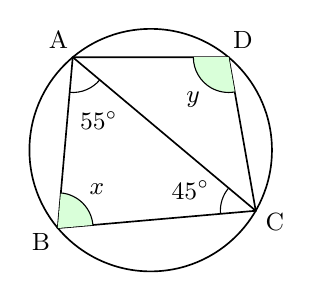
\begin{tikzpicture}[scale=1.40, line width=0.6pt]
  \draw (0.000,0.000) circle (1.100);
  \draw (-0.707,0.843) -- (-0.843,-0.707) -- (0.953,-0.550) -- (0.707,0.843) -- cycle;
  \draw (-0.707,0.843) -- (0.953,-0.550);
  \draw[line width=0.4pt] (-0.735,0.524) arc[start angle=-95.000, end angle=-40.000, radius=0.320];
  \node[font=\small, inner sep=0.5pt] at (-0.470,0.270) {$55^\circ$};
  \draw[line width=0.4pt] (0.707,-0.344) arc[start angle=140.000, end angle=185.000, radius=0.320];
  \node[font=\small, inner sep=0.5pt] at (0.361,-0.364) {$45^\circ$};
  \fill[green!15] (-0.843,-0.707) -- (-0.524,-0.679) arc[start angle=5.000, end angle=85.000, radius=0.320] -- cycle;
  \draw[line width=0.4pt] (-0.524,-0.679) arc[start angle=5.000, end angle=85.000, radius=0.320];
  \node[font=\small, inner sep=0.5pt] at (-0.489,-0.354) {$x$};
  \fill[green!15] (0.707,0.843) -- (0.387,0.843) arc[start angle=180.000, end angle=280.000, radius=0.320] -- cycle;
  \draw[line width=0.4pt] (0.387,0.843) arc[start angle=180.000, end angle=280.000, radius=0.320];
  \node[font=\small, inner sep=0.5pt] at (0.386,0.460) {$y$};
  \node[font=\small, inner sep=1.5pt] at (-0.836,0.996) {A};
  \node[font=\small, inner sep=1.5pt] at (-0.996,-0.836) {B};
  \node[font=\small, inner sep=1.5pt] at (1.126,-0.650) {C};
  \node[font=\small, inner sep=1.5pt] at (0.836,0.996) {D};
\end{tikzpicture}
